In this project, we focus on link prediction task for knowledge graphs 
(KGs). Given incomplete triple in a KG \((h, r, ?)\) or \((?, r, t)\), 
the goal is to predict the missing entity, either it is head \(h\) 
or tail \(t\), where \(h, t \in E\) and \(r \in R\), E denotes set of 
entities, R denotes set of relations. The model that we used follows 
KICGPT \cite{wei2023kicgpt} with modification on the LLM used. 

\subsection{Architecture}
\label{sec:method:architecture}

\begin{figure}
    \centering
    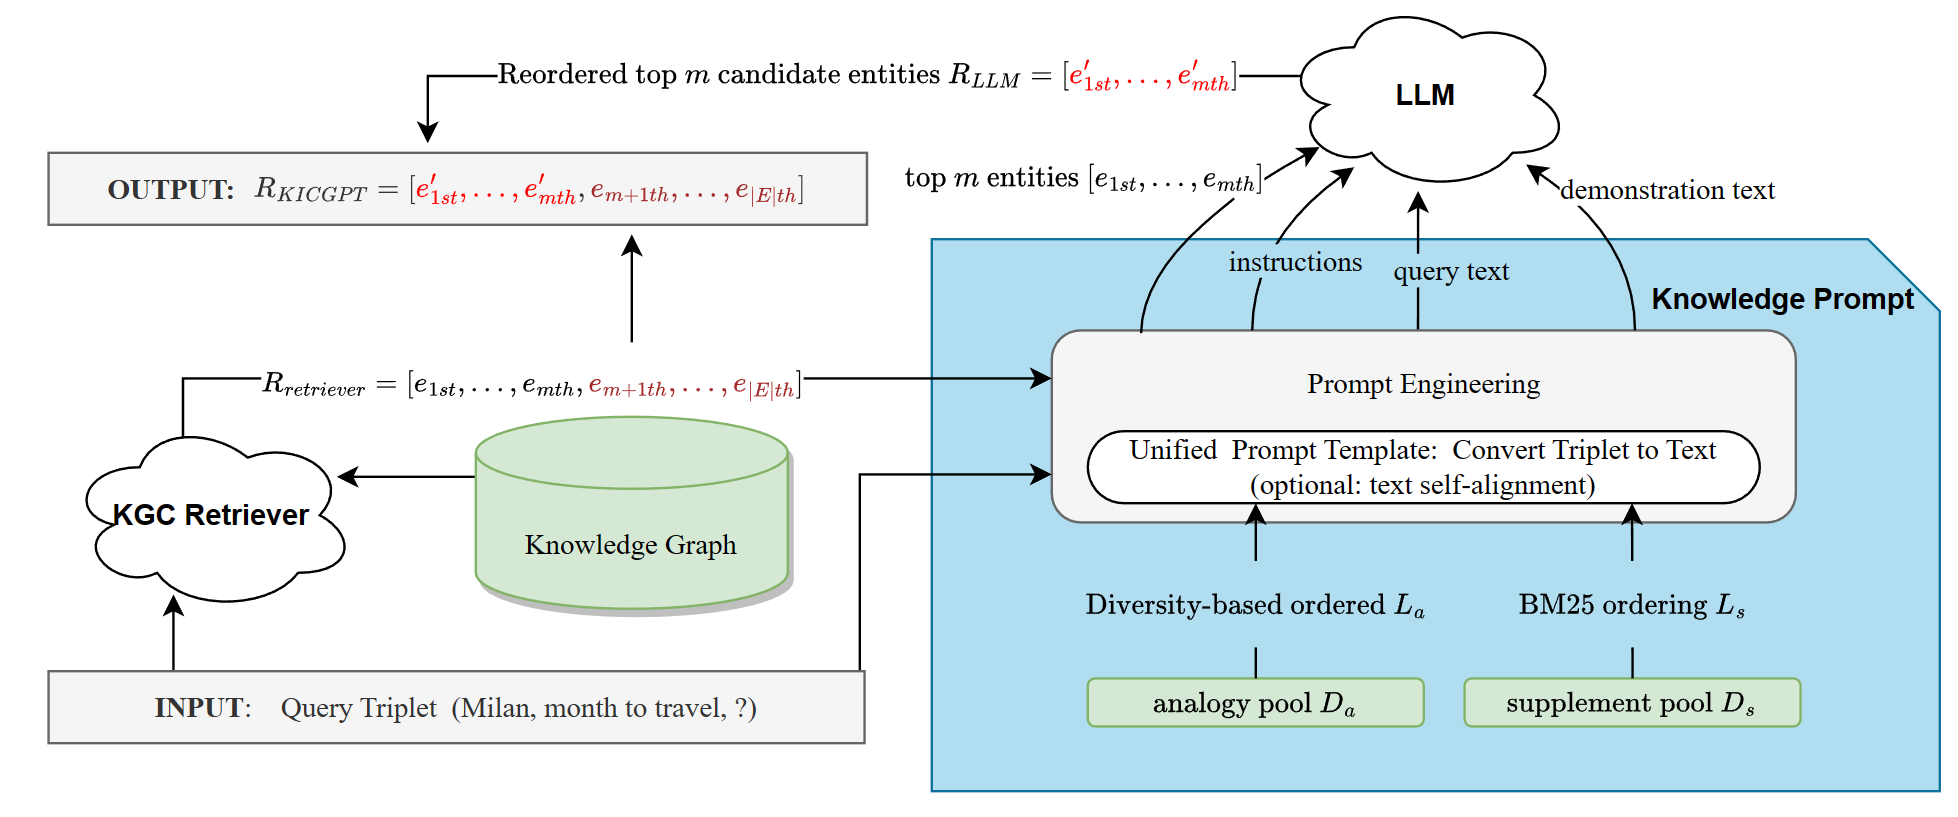
\includegraphics[width=0.8\textwidth]{figures/arc3.png}
    \caption{KICGPT Architecture \cite{wei2023kicgpt}}
    \label{fig:KICGPTarchitecture}
\end{figure}

KICGPT primarily covers three main components as can be seen in Figure 
\ref{fig:KICGPTarchitecture}, which are a triple-based KGC retriever, 
the Knowledge Prompt, and a LLM. For each query triple \((h, r, ?)\), 
the KGC retriever retrieves the score of \((h, r, e)\) for each entity 
\(e \in E\) in descending order 
\(R_{retriever} = [e_1, e_2, ..., e_{|E|}]\). 
Using prompt engineering in the Knowledge Prompt, LLM performs reranking 
of the top \(m\) entities 
\(R_{LLM} = [e^{'}_1, e^{'}_2, ..., e^{'}_m]\). Finally, KICGPT will 
output final ranking of top m entities from the LLM and the rest of
the entities from the KGC retriever 
\(R_{KICGPT} = [e^{'}_1, e^{'}_2, ..., e^{'}_m, e_{m+1}, ..., e_{|E|}]\)

\subsubsection{Knowledge Prompt}
Knowledge Prompt is introduced in KICGPT as in-context learning
strategy to provide context to the LLM by integrating part of the KG
into the demonstration. There are two pools of triples in the 
demonstration, analogy pool \(D_a\) and supplement pool \(D_s\). 
To help the LLM understand the query triple, the analogy pool contains 
triples with the same relation \(r\) as the query \((h, r, ?)\), 
\(D_a = \{(e^{'}, r, e^{"}) \in G_{train} \cup G_{valid} \mid e, e^{"} \in E\}\).
In addition, the supplement pool contains triples with one of its entity 
(tail or head) is the same as the query's head \((h, r, ?)\),
\(D_s = \{(h, r, e^{'}) \in G_{train} \cup G_{valid} \mid r^{'} \in R, e^{'} \in E\} \cup
\{(e^{'}, r, h) \in G_{train} \cup G_{valid} \mid r^{'} \in R, e^{'} \in E\}\).
This is to provide additional information of the query's head to the LLM.

The ordering of the demonstration is important as it affects the LLM performance.
For the analogy pool, each entity starts with a zero counter. 
A random triple from \(D_a\) is chosen first, increasing its entities'
counters by 1. Next, the triple with the lowest summed counter values 
is selected, repeating until all triples are used. The final ordered 
list is denoted \(L_a\). The supplement pool \(D_s\) provides additional context 
for the query's head entity \(h\), prioritizing relevant demonstrations. 
To achieve this, triples in \(D_s\) are ranked based on their BM25 scores, 
which measure their textual similarity to the query. The final ordered list, 
denoted \(L_s\), includes all triples from \(D_s\).

\subsubsection{Prompt Engineering}

To adapt structured triples into natural language input, KICGPT uses 
a unified prompt template, ensuring consistent formatting for queries 
and demonstrations. The interaction with the LLM follows a multi-round 
process. First, the responsibility description stage clarifies the LLM's 
role in ranking candidate answers. Next, in the question and demonstration 
description stage, the query is presented along with an explanation of 
two demonstration types: analogy-based and supplementary examples.

In the demonstration input stage, batches of demonstrations from the 
analogy \(L_a\) and supplement \(L_s\) pools are provided, repeated 
as much as the token limit allows to maximize knowledge inclusion. 
Finally, during the final query and re-ranking stage, the LLM ranks 
the top-m candidate entities, producing an ordered list \(R_{LLM}\), 
which replaces the top-m results from the retriever to generate the 
final answer.